\section{Evaluation}

\subsection{Input Pipeline with multiple GPUs}

\subsection{Charades Classification without TOV Pre-Training}

\begin{figure}[H]
    \begin{subfigure}[c]{\textwidth}
    \centering
    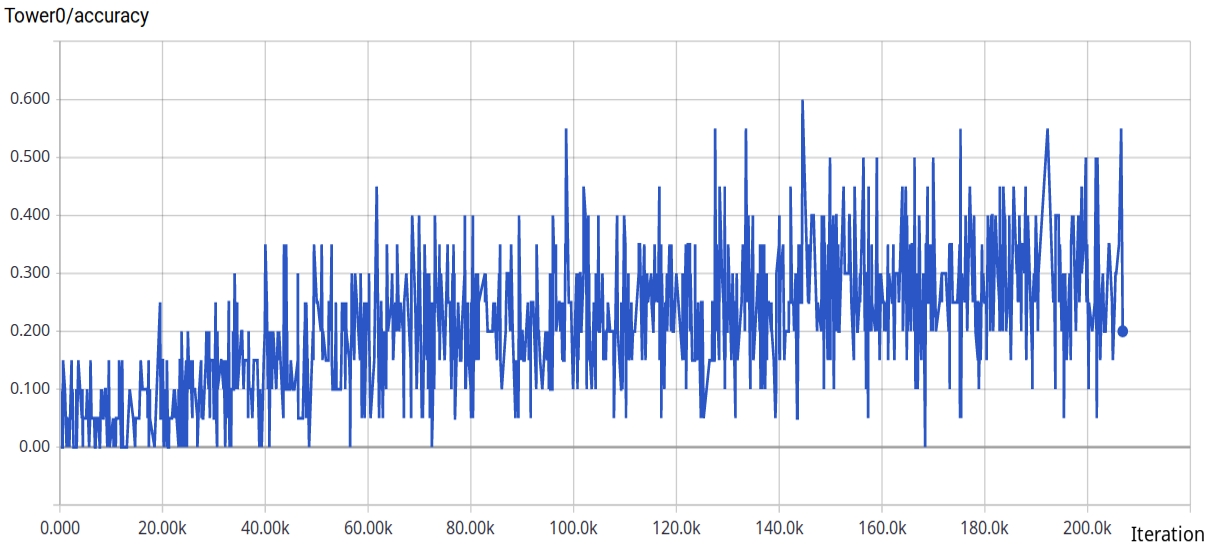
\includegraphics[width=\textwidth]{img_evaluation/tower0accuracy}
    \subcaption{<+captiontext+>}
    \end{subfigure}
    \begin{subfigure}[c]{\textwidth}
    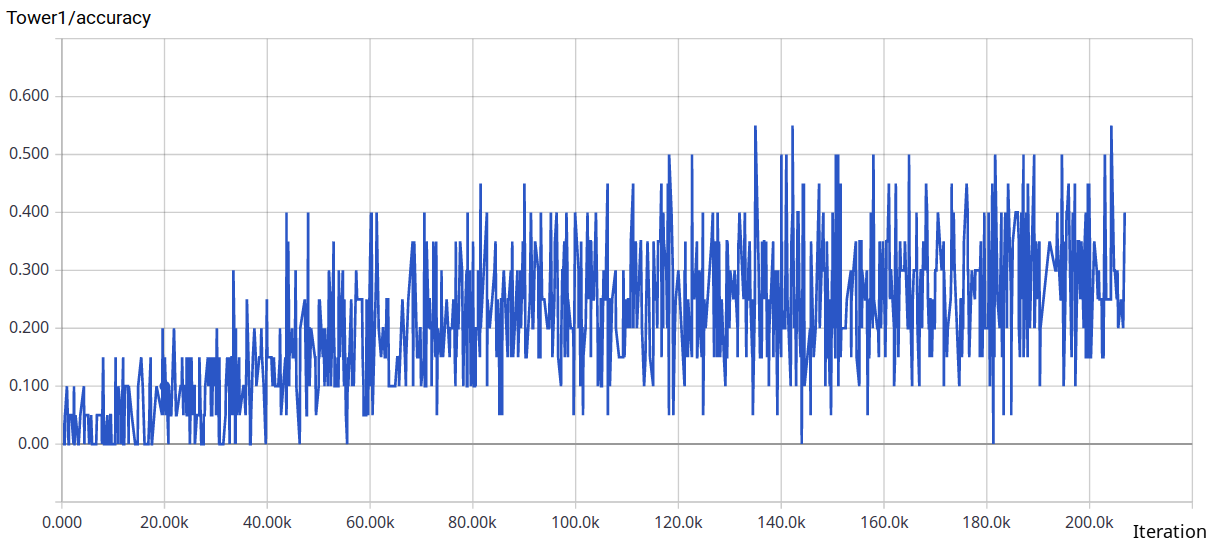
\includegraphics[width=\textwidth]{img_evaluation/tower1accuracy}
    \subcaption{<+captiontext+>}
    \end{subfigure}<++>
\label{fig:<+label+>}
\end{figure}<++>

\begin{figure}[H]
    \begin{subfigure}[c]{\textwidth}
    \centering
    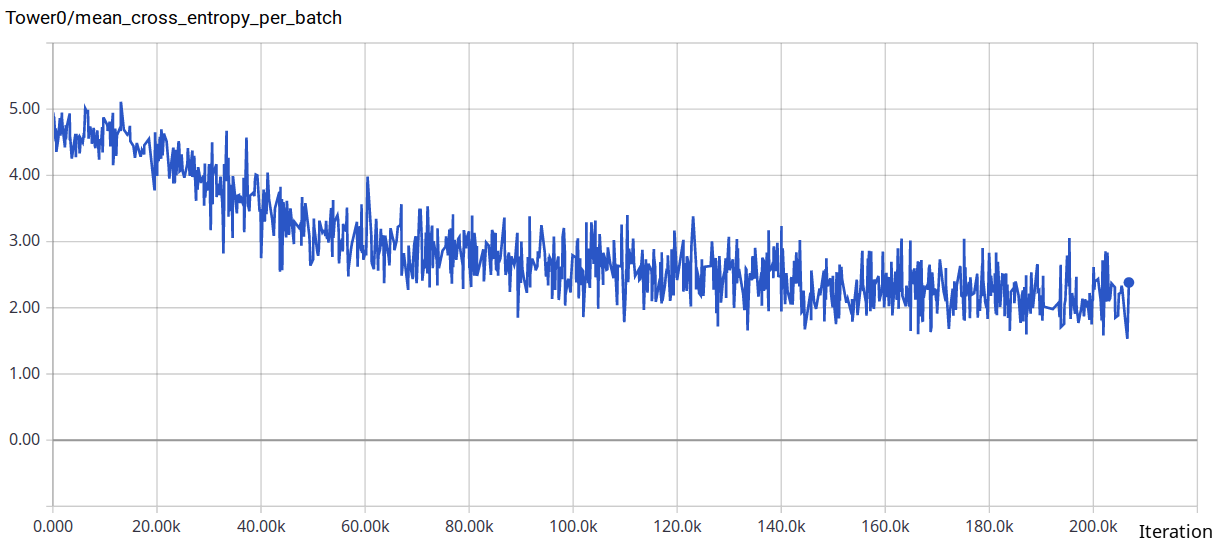
\includegraphics[width=\textwidth]{img_evaluation/tower0crossentropy}
    \subcaption{<+captiontext+>}
    \end{subfigure}
    \begin{subfigure}[c]{\textwidth}
    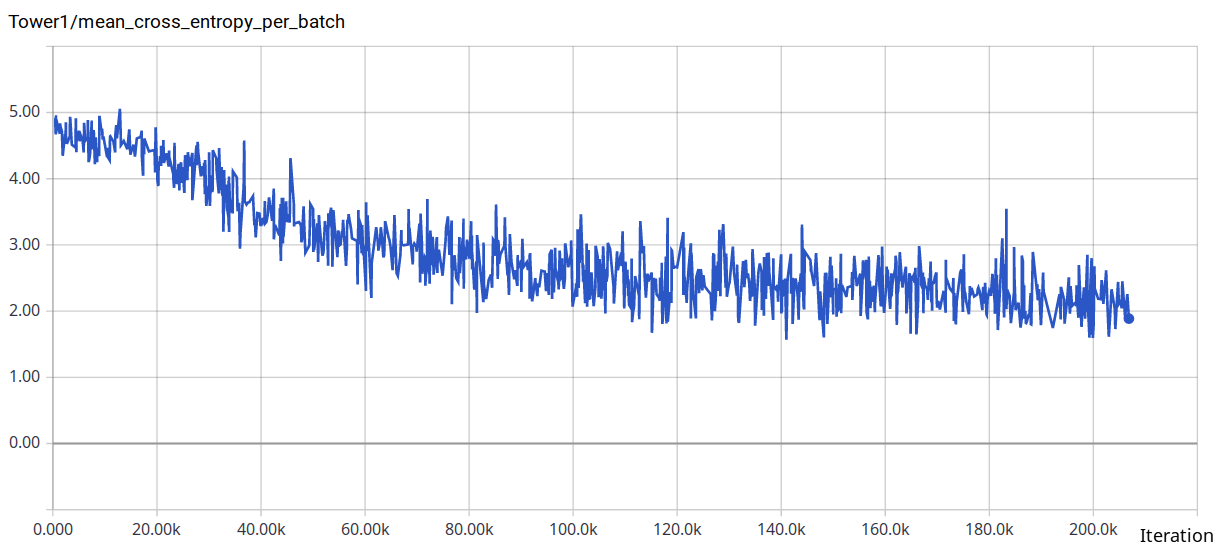
\includegraphics[width=\textwidth]{img_evaluation/tower1crossentropy}
    \subcaption{<+captiontext+>}
    \end{subfigure}<++>
\label{fig:<+label+>}
\end{figure}<++>


\subsection{UCF-101 Classification without Pre-Training}


\subsection{Pre-Training on Kinetics}


\subsection{Charades Classification with Pre-Training}


\subsection{UCF-101 Classification with Pre-Training}


\section{Conclusion}


\section{Future Directions}
\label{sec:future_work}
Incorporate domain bias into the learning/classification pipeline.

A human detector could be incorporated to provide the learning system with more relevant training clips.

See attention-networks?
